% This example An LaTeX document showing how to use the l3proj class to
% write your report. Use pdflatex and bibtex to process the file, creating 
% a PDF file as output (there is no need to use dvips when using pdflatex).

% Modified 

\documentclass{l3proj}
\usepackage{datetime}
\usepackage{graphicx}

\begin{document}
\title{Algorithm Animator}
\author{Arthur Bigeard \\
		Alexander Ferguson \\
		Andrew Gibson \\
		Gediminas Leikus \\
		Liam Bell}
\usdate
\date{\today}
\maketitle
\begin{abstract}

For teaching purposes it is useful to be able to animate algorithms and produce a visual representation of how they work. The basic idea is to use a diagrammatic representation of a data structure, for example an array or a tree, and illustrate the algorithm step by step, showing how the data structure is accessed and changed. The aim of this project is to design and implement a system for animating algorithms. There are at least two possible approaches. One is to design and implement a simple programming language in such a way that all programs are animated while being executed. Another is to design and implement an API for animations, so that an existing program (in Java, for example) can be animated by inserting calls to your library. The system should be as general as possible in the sense of supporting a range of styles of algorithm, and should be demonstrated by producing a range of animations of standard algorithms. It would also be useful to be able to 
capture the animation in a form that can be viewed independently of your system, for example as a sequence of HTML pages or a Flash animation.

\end{abstract}
\educationalconsent
\tableofcontents
%==============================================================================
\chapter{Introduction}
\label{intro}

Alice was beginning to get very tired of sitting by her sister
on the bank and of having nothing to do: once or twice she had peeped into
the book her sister was reading, but it had no pictures or conversations in
it.

\begin{figure}
\begin{center}

\includegraphics[width=7cm]{figures/alice}
\end{center}
\caption{Behind it was a little door}
\label{fig:alice}
\end{figure}

Alice opened the door and found that it led into a small passage, not much
larger than a rat-hole: she knelt down and looked along the passage into
the loveliest garden you ever saw.

%==============================================================================
\chapter{Design}
\label{design}

\section{Use cases}
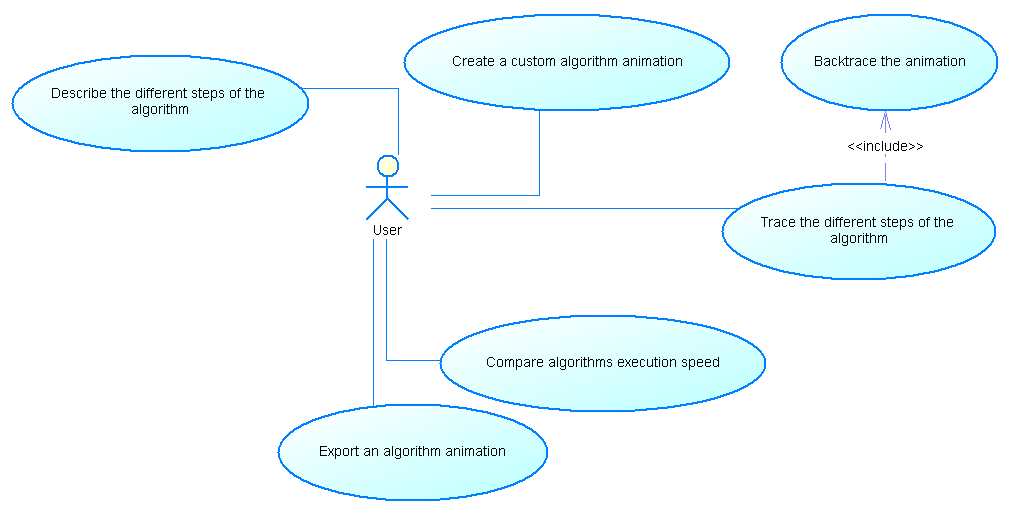
\includegraphics[width=115mm]{images/useCases.png}

Our use cases are meant to illustrate the main functionalities of our system. Using our API's, users will
be able to:
\begin{itemize}
\item Create custom algorithm animations on Linked Lists, Arrays and Heaps data structures
\item Display descriptions of the various steps of the animation as it processes
\item Navigate freely between the different steps of the animation backwards or forwards
\item Export animations in an executable format
\end{itemize}
\section{Components}
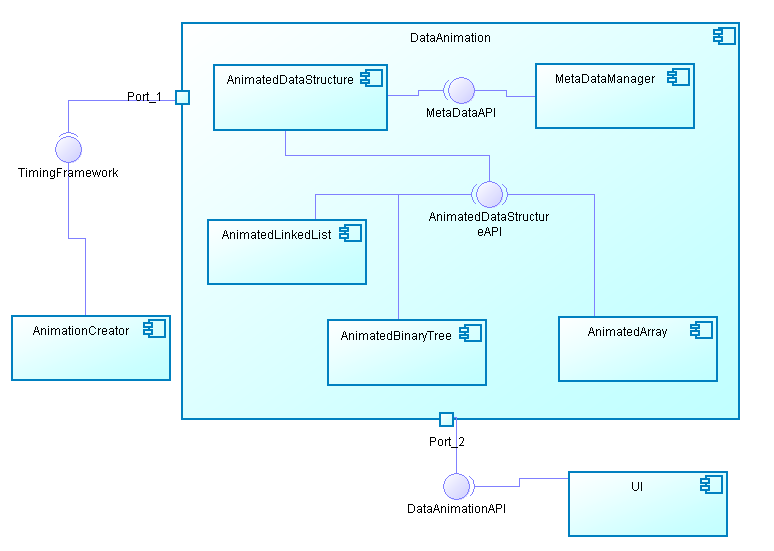
\includegraphics[width=115mm]{images/componentDiagram.png}

\section{Classes}
\subsection{AnimatedDataStructure Component}
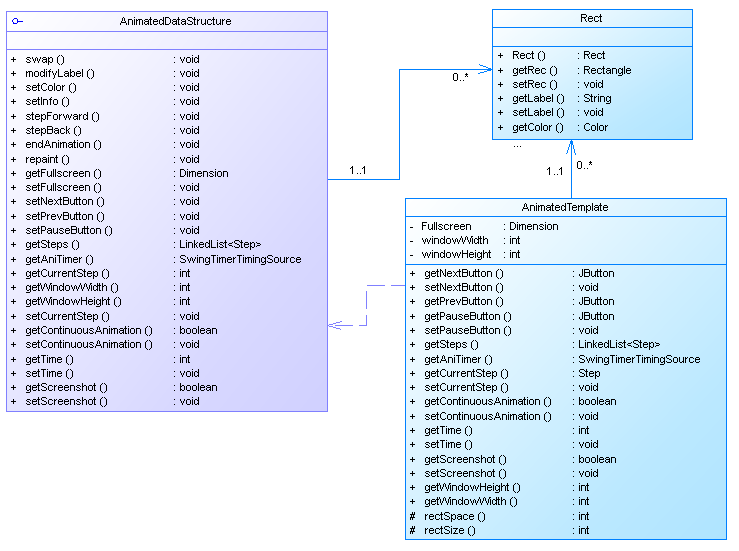
\includegraphics[width=115mm]{images/animatedDataStructureDiagram.png}

This diagram shows the component design of the system and their dependencies. The core of the system is the DataAnimation component,
which is relying on the Animation creating TimingFramework API, provided by a component labeled AnimationCreator.
The DataAnimation component is an aggregate of the components required to create a complete data animation, AnimatedDataStructure and MetaDataManager, and the data structure animation components
resulting from the use of the first two components. Our animations are called by the UI component to enable displaying them.
We can infer from this diagram the system architecture is a facade architecture, where the UI component is the facade component.

\subsection{AnimatedArray Component}
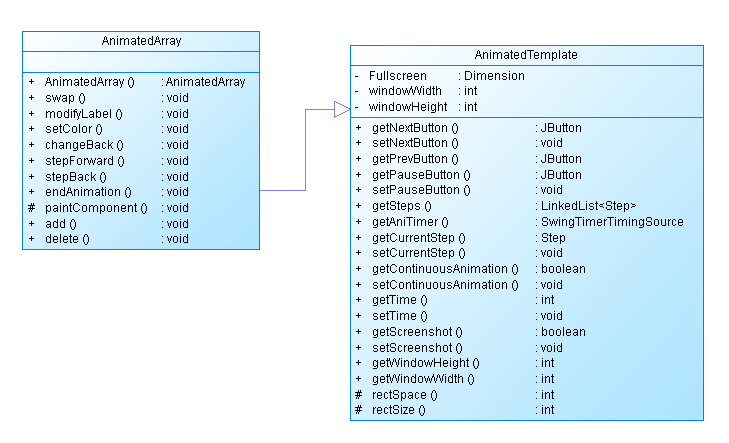
\includegraphics[width=115mm]{images/arrayDiagram.png}
\subsection{AnimatedLinkedList Component}

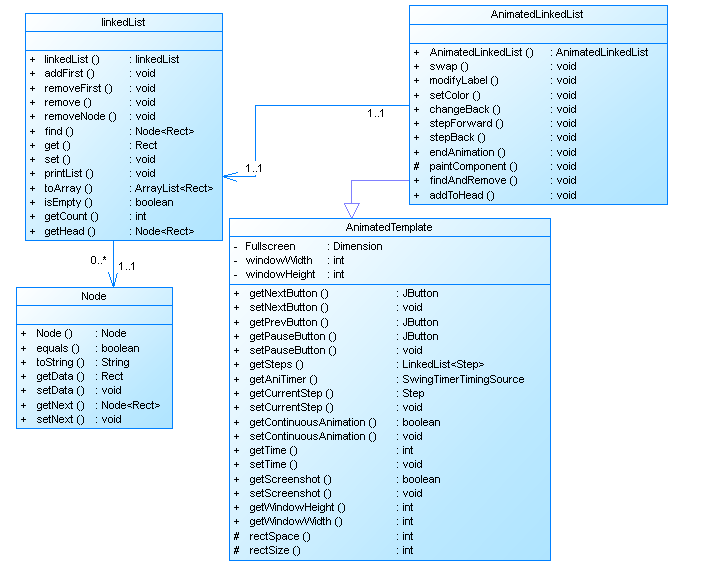
\includegraphics[width=115mm]{images/linkedListDiagram.png}
The AnimatedLinkedList data structure requires additional classes to store the Rect objects in a way that is coherent to the data structure.
The Rect's are stored in a custom linked list data structure implemented such that manipulating the data stored in the list will also update the display of
the linked list.
\subsection{AnimatedHeap Component}
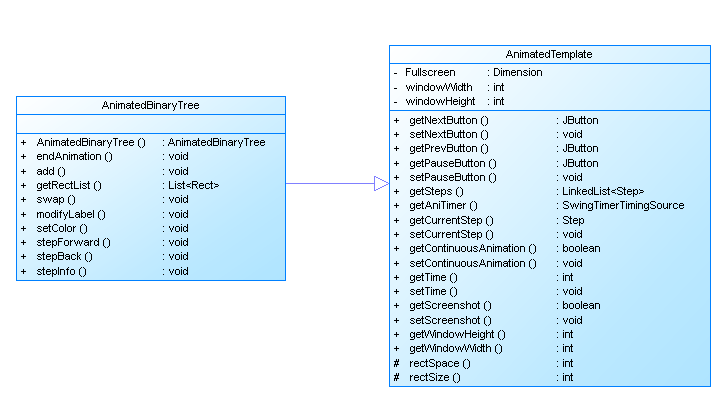
\includegraphics[width=115mm]{images/heapDiagram.png}
\subsection{MetaDataManager Component}
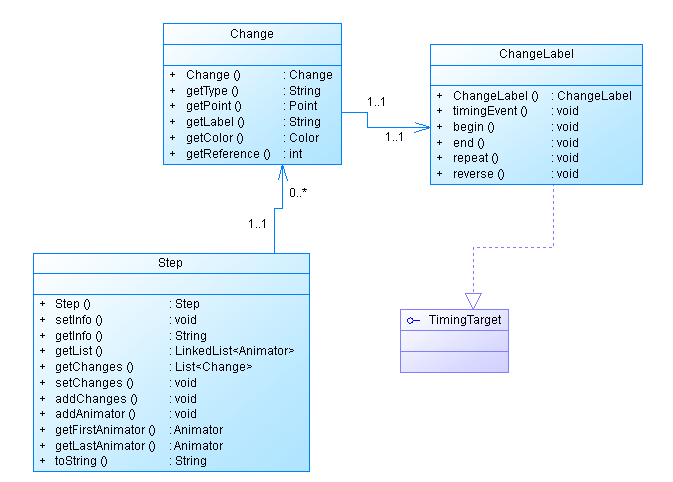
\includegraphics[width=115mm]{images/metaDataDiagram.png}
The MetaDataManager component provides a set of classes and functions meant to store the steps and step informations of the animations. The user manipulates
those data through the public animating calls made in the different data structures' classes.
\subsection{UI Component}
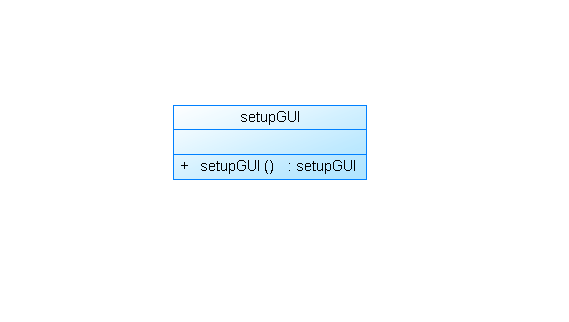
\includegraphics[width=115mm]{images/UIDiagram.png}
%==============================================================================
\chapter{Implementation}
\label{impl}

In this chapter, we describe how the implemented the system.

%------------------------------------------------------------------------------
\section{User Interface}

Blah blah blah
Blah blah blah
Blah blah blah
Blah blah blah

% - - - - - - - - - - - - - - - - - - - - - - - - - - - - - - - - - - - - - - -
\section{Problems Encountered}
\subsection{Arthur Bigeard}
Once our team got familiar with the TimingFramework, the application started rapidly growing and quickly our first animated algorithms were produced. 
On early stages of the animation display, we figured several features should be added to the display to increase the potential of our animations, features including:
\begin{itemize}
\item Labelling the steps of the animation
\item Navigating through steps from a list
\item Resizing dynamically the window to fit several animation demonstrations on a screen
\item Dynamically changing the speed of the animation using simple Speed Up/Speed Down JButtons
\end{itemize}

Introducing dynamic features to the animation constituted a challenge on several levels:
\begin{itemize}
\item performance-wise : the animation approach taken with the TimingFramework requires creating several objects per step; our approach of algorithm animation is such that animation are splitted
in a multitude of atomic steps and therefore consume a lot of memory
\item algorithm-wise : dynamic features require to look up and modify crucial data to the animation, where corruption of those data would lead to display inconsistencies or program termination
\item boundary-wise : our animations are limited by the animation framework we're using, the TimingFramework; we cannot implement what the TimingFramework cannot do
\end{itemize}

To illustrate better the challenges involved in implementing dynamic features, here is a list of data potentially subject to changes:
\begin{itemize}
\item Rect's and Rectangle's x/y coordinates and edge size
\item Step's Change Linked List 
\item Change's changed Object reference
\item Animation triggers, the Animator objects provided by the TimingFramework
\item setupGUI
\end{itemize}

Attempting to implement dynamic speed changing of the animation demonstrates very well the limits of the TimingFramework and our implementation:
\begin{figure}
\begin{center}
\begin{verbatim}
Step s = new Step(); // create a new step
// Create animation for showing information on what's happening
String information;
if (info == "") {
    information = "Swapping index " + a + " (" + rect_list.get(a).getLabel() + 
        ") " + " with index " + b + " (" + rect_list.get(b).getLabel() + ")"; // create the string
} else {
    information = info;
}
s.setInfo(information); // add it to the step
// Change information
s.addAnimator(new Animator.Builder().setDuration(1, TimeUnit.MILLISECONDS)
    .build(), s.getFirstAnimator()); // create an animator for this, which 
                                     //we could use to trigger this change
s.getLastAnimator().addTarget(new ChangeLabel(this, information, this));
// create a timing target to change the label when the animation starts	
// Create the Animators and PropertySetters (what should the animation change 
// the property from what to what) for swapping rects
s.addAnimator(new Animator.Builder().setDuration(time, TimeUnit.MILLISECONDS)
	.build(), s.getFirstAnimator()); // we want this Animator to start the same
// time the first Animator in the step does
s.getLastAnimator().addTarget(PropertySetter.getTarget(rect_list.get(a), 
	"currentY", rect_list.get(a).getRec().y, rect_list.get(a).getRec().y+rectSpace()));
s.addAnimator(new Animator.Builder().setDuration(time, TimeUnit.MILLISECONDS)
	.build(), nextBtn); // we want this Animator to start straight after the 
	// last Animator finishes. This is how it's done just now
s.getLastAnimator().addTarget(PropertySetter.getTarget(rect_list.get(a), "currentX", rect_list.get(a).getRec().x, rect_list.get(b).getRec().x)); 
s.addAnimator(new Animator.Builder().setDuration(time, TimeUnit.MILLISECONDS).build(), nextBtn);
s.getLastAnimator().addTarget(PropertySetter.getTarget(rect_list.get(a), "currentY", rect_list.get(a).getRec().y+rectSpace(), rect_list.get(a).getRec().y));		
//rect 2
s.addAnimator(new Animator.Builder().setDuration(time, TimeUnit.MILLISECONDS).build(), s.getFirstAnimator());															// we want this Animator to start the same time the first Animator in the step does
s.getLastAnimator().addTarget(PropertySetter.getTarget(rect_list.get(b), "currentY", rect_list.get(b).getRec().y, rect_list.get(b).getRec().y-rectSpace()));
s.addAnimator(new Animator.Builder().setDuration(time, TimeUnit.MILLISECONDS).build(), nextBtn);
s.getLastAnimator().addTarget(PropertySetter.getTarget(rect_list.get(b), "currentX", rect_list.get(b).getRec().x, rect_list.get(a).getRec().x));
s.addAnimator(new Animator.Builder().setDuration(time, TimeUnit.MILLISECONDS).build(), nextBtn);
s.getLastAnimator().addTarget(PropertySetter.getTarget(rect_list.get(b), "currentY", rect_list.get(b).getRec().y-rectSpace(), rect_list.get(b).getRec().y));
// Trigger for a continuous animation
s.addAnimator(new Animator.Builder().setDuration(1, TimeUnit.MILLISECONDS).build(), nextBtn);
s.getLastAnimator().addTarget(new ContinuousAnimation(currentStep+1, this));
// Log the changes in the Step
s.addChanges(new Change("swap", rect_list.get(a), rect_list.get(a).getRec().x, rect_list.get(a).getRec().y));
s.addChanges(new Change("swap", rect_list.get(b), rect_list.get(b).getRec().x, rect_list.get(b).getRec().y));
\end{verbatim}
\end{center}
\caption{Sample code from the AnimatedArray swap function}
\label{fig:swap}
\end{figure}

As you can see on this sample piece of code, the "core" of the animation, the Animator objects, are passed a static time value. We're keeping track
of the Animators in a LinkedList stored in the corresponding step of the animation. A basic approach to the feature would be to simply browse every single
Animator objects in our Step and modify the time value stored in the trigger using a simple speed ratio going from 0.25 to 4 for example. However, and this
is where the TimingFramework failed to our expectations, once created, the Animator objects cannot be modified. Hence, it is not possible from this approach
to implement dynamic speed change to the system.

At this stage, it was still possible to implement dynamic speed change to the animation. If we cannot modify our Animators, the logical next step to the solution
is the re-create the Animators instead of modifying them. This alternate solution is extremely constraining:
\begin{itemize}
\item performance-wise : Re-creating the Animators involve 3 steps: browsing steps, destroying animators, re-creating them.
\item algorithm-wise : This solution requires heavy coding. While the first solution would only require to modify a time field, this solution requires to look up the type of
Step we're currently modifying and the type of data structure we're animating in order to re-create the Animators properly
\item requirements-wise : Destroying the Animators object would obviously require us to restart the animation from the beginning; not only this is not the expected behaviour from
a speed change button, this solution might also cause the application to hang due to the heavy object manipulation overhead
\end{itemize}

Due to too heavy constraints this solution was quickly dropped. With the current analysis of the implementation requirements for this feature, only one solution could reasonably be infered:
static speed changing. As you've seen on (\ref{fig:swap}), we can specify the duration of the animation when creating the Animators; the solution adopted was that the user can specify his own time unit
when making calls to create an algorithm animation. 


Attempting to implement dynamic window resizing also showed the limits of our own implementation and especially of the Step management system.
Although this solution was almost fully coded and working on a first and long attempt, we decided to give up on it for a cleaner, easier static resizing 
solution.
Implementing this feature was very challenging regarding to the consistency of the Step data stored by the system. To get a better idea of the issues involved
in dynamic resizing, here's a reminder of the potential data involved in resizing:
\begin{itemize}
\item Steps
\item Rects and Rectangles
\item Changes
\item setupGUI
\end{itemize}

Two implementations can be suggested for this feature; they both have their own perks and withdraws:
\begin{itemize}
\item Keeping a window width/height ratio relative to a fullscreen size from which the original x,y coordinates and size of the elements
are calculated. The window width/height ratio would simply be used to adapt those x,y coordinates and element size. While this solution is very simple
to code, it may lead to severe data inconsistency: using has a strong impact on the data precision, therefore, an expectable consequence from this implementation
is unaligned elements. However, it is important to notice that the performance overhead is neglectable.
\item Re-creating the data involved in window resizing. Practically, this solution requires a lot more coding. It is extremely unefficient for the same reasons explained
on the dynamic animation speed changing. It would also require to restart the entire animation each time the window is resized.
\end{itemize}

The second solution can clearly be dropped due to its obvious disadvantages. In the process of coding, this is how I went about defining how I may implement dynamic window resizing.

The first solution was implemented; as expected, resizing resulted in unaligned elements. Usually, the scaling of the elements would be inconsistent from a range of 5 to 20 pixels.
I have considered the eventuality of adding a scaling function to align the elements after the resizing process and after each step. Again, this fix has huge disadvantages: scaling elements would be done
regardless to the position of the elements on the window, and multiple resizing may result in elements gradually moving up and down the window, and in the worst cases litterally working all their way up or down the window.
Why? Simply because scaling the elements would require to move them all up or down the window. Elements would no longer be centered. 
Again, performance-wise, this solution increases a lot the operations required to run steps on the animation.

Our team discussed the need for dynamic resizing, to either justify dropping this feature or keeping it and improving it so that it works perfectly.
We've decided to drop dynamic resizing for static resizing on the following assumptions:
\begin{itemize}
\item The user is unlikely to resize his window on a regular basis.
\item The user aims to demonstrate algorithms graphically. Where demonstration is involved, preparation is involved too. We can reasonably suppose that our end-users
will choose a fixed window size for their demonstration, if not fullscreen size, and keep the window to that size until the end of the animation. Therefore, determining the window
size statically will satisfy the need for users to determine a custom animation window size. 
\subsection{Alexander Ferguson}
\subsection{Andrew Gibson}
\subsubsection{The selection of a suitable animation framework}

During the beginning of the project, I was assigned to the research area where I was to examine a suitable graphics framework that could assist the team in building a solid animation API for our end users. During my research, I found there were several popular graphics frameworks for assisting with animation alongside Java applications, typically integrated through the use of compiled classes within a Java archive (.jar).

The range of frameworks proved problematic, given that it was most suitable to select a single framework to build with, otherwise there would be serious inconsistencies between developed applications (as they differ in their functionality) We established a simple set of fundamental criteria for selection as follows:
\begin{itemize}
	\item The framework should offer a fully functional API, of which can be accessed by our code in order to build animation.
	\item It should provide some degree of control, so that our own API can display dynamic movement and precision.
	\item It should be able to be in-cooperated into an integrated development environment (IDE) for group production during the implementation stage.
\end{itemize}

After careful research, I found three separate candidates for animation production with Java. In order to justify a suitable approach, each framework was considered separately to assess desirable characteristics and identify potential flaws. 

\underline{\textbf{Timing-Framework:}}

The Timing Framework was found on Java.net, a place for Java based libraries and extensions (\cite{website:TimingFramework}). It features controlled timing and ease of animation.

\textit{Advantages:}
\begin{itemize}
	\item The library is multi-threaded and concurrently safe. This prevents us from having to worry about complex synchronization issues between multiple application threads (as our animation software will utilise several threads for handling graphical changes independently)
	\item Uses less memory, putting a smaller load on systems with limited memory, allowing more applications to execute at once. 
	\item Offers an extensive API, giving us the ability of more control and functionality over our animations.
	\item Supportive of Swing and SWT development, for flexibility over a suitable distribution
	\item Its functionality can produce smooth, complex and controlled animation, useful for providing sufficient detail to our users in an orderly fashion.
	\item Can be in-cooperated easily into an existing Eclipse project (a solid Java development IDE, which all the team have good knowledge of)
\end{itemize}

\textit{Disadvantages:}
\begin{itemize}
	\item The API is detailed and complex in areas, which may invoke a steep learning curve.
	\item Swing examples documented are rather vague, and information given in a relevant PDF chapter is out dated.
\end{itemize}

\underline{\textbf{Java-FX:}}

Java-FX was found on the Oracle technology website (\cite{website:JavaFX}) it features UI based accelerated graphics. Its control is timeline based.

\textit{Advantages:}
\begin{itemize}
	\item Like the Timing-Framework, it also uses concurrently safe libraries.
	\item Potentially less complex to learn, given that Oracle have provided a more comprehensive set of documentation, including video tutorials.
\end{itemize}

\textit{Disadvantages:}
\begin{itemize}
	\item Newer libraries are not supported within Eclipse. This isn’t useful to us as a team as our preferred development environment is Eclipse. It is more suited to the Netbeans IDE, which we aren’t familiar with.
	\item It is more oriented towards web-based user interface development, typically within business. The goal of our application does not support this business approach, and focuses on the aspects of animation rather than an interactive interface with less emphasis on complex animation techniques.
\end{itemize}

\underline{\textbf{Trident:}}

Like the Timing-Framework, this was also found as part of a Java.net library development (\cite{website:Trident}) it’s focused entirely on timelines, namely duration and object changes across such durations represented by keyframes.

\textit{Advantages:}
\begin{itemize}
	\item Supports Swing and SWT development
	\item Allows multiple timeline events to be run and scheduled at any one time (multiple animations)
	\item Conceptually, it is straight forward and approachable; timelines represent the course of the animation and the keyframes the alterations to animation objects.
\end{itemize}

\textit{Disadvantages:}
\begin{itemize}
	\item Little documentation and not completely approachable as a result.
	\item It doesn’t seem to fully support concurrency as part of its API. To give an example, the code below taken from the documentation section on timelines demonstrates parallel timeline objects competing for shares properties(http://www.pushing-pixels.org/2009/06/25/trident-part-8-timeline-scenarios.html)
\end{itemize}

\begin{figure}
\begin{center}
\begin{verbatim}
        synchronized (this.circles) {
            circles.add(circle);
        }
        scenario.addScenarioActor(timeline);
    }
return scenario;
}...
public void paint(Graphics g) {
    synchronized (this.circles) {
        for (SingleExplosion circle : this.circles) {
            circle.paint(g);...
\end{verbatim}
\end{center}
\caption{Make a description up, Andrew}
\label{fig:frameworkExamples}
\end{figure}

In both examples \ref{fig:frameworkExamples} it can be seen that intrinsic locking is needed because of shared properties between objects. This adds a considerable degree of complexity to the framework, and would inevitably increase development time through the bugs and issues raised from concurrent access. For instance, if two objects were competing for shared animation data, and writing to it simultaneously, this would create unexpected behaviour. We would have to consider thread safe concepts alongside our own application complexity.

To conclude, we felt that the Timing-Framework offered the best and most approachable set of features. It provides multiple, dynamic animation techniques; with an emphasis on the animation itself as supposed to client designed web applications. It is also concurrent, which is hugely important as it draws a significant amount of complexity out the project. The animations we create will have their own threads delegated to tasks within the framework. The precision of control it offers is also an attractive trait, allowing us to build highly tweaked and well performing animations to our end users. 

Of course, the Timing-Framework is probably the most complex, but the positives most certainly outweigh the negative aspects. The analysis of these separate frameworks proved to be very useful in that sense, standing out as an important design choice that most likely would of saved us more development time in comparison to the other frameworks.

\subsubsection{Development of Animated Linked Lists}

For part of the project I worked on the development of linked lists. I utilised the trigger design that Gediminas created for scheduling animations in a step based fashion, such that the user can step through each part individually. To begin with, I created a linked list class with generic nodes, which would eventually function as objects associated with animations (class of type Rect). I represented the linked list as an array of these generic node objects. There were several problems I encountered when attempting to in-cooperate the step-based animation classes into my own code. It became apparent that some of the step-based algorithms involved with the successfully built Animated-Array class didn’t directly translate to my own Animated-Linked-List structure. A step in this sense is represented as a series of animations, as noted before.

The intention of my Animated-Linked-List class was to offer specific algorithmic operations associated with linked list data structures. The issue I encountered was attempting to implement a suitable algorithm to locate and remove all instances of a specific node in the list. Addressing the step-based approach for this algorithm, it was required that the deletion of each found copy of the node was represented as a step. Initially, I developed the algorithm which directly removed the found occurrence from the list of objects.

\begin{figure}
\begin{center}
\begin{verbatim}
while(node.getNext() != null && !(node.getData().getLabel().equals(i))){
    prev = node; //pointer to previous node
    setColor(count,Color.RED,"Changing color to red");
    setColor(count,Color.BLUE,"Changing color to blue");
    node = node.getNext();
    count++;
}
anim.setColor(count,Color.GREEN,"Changing color to green");
anim.setColor(count,Color.WHITE,"Changing color to white");
(**) prev.setNext(node.getNext());   //joins the pointer for the prev element after the to be deleted node
(**) rect_list.removeNode(node); //removes this node
\end{verbatim}
\end{center}
\caption{Make a description up, Andrew}
\label{fig:linkedListsExample}
\end{figure}

This proved to be problematic. Once executed, the animation would display the deleted node to the user, before they have even stepped through the animation and eventually reached the deletion of the found node. The early implementation of the problem highlights this issue (\ref{fig:linkedListsExample}).

This section of code (\ref{fig:linkedListsExample}) represents a linear scan across each of the list’s pointers, until the required node is found. When a node is found, it is highlighted, and subsequently deleted. The last two lines indicated by (**) in this piece of code highlight the issue. Although the overall method for locating and removing a node is represented as a step, the changes made directly to the linked list object (represented here as rectlist) are not stored in any structures that allow the user to step through. Hence, when the application is executed, these adjustments are already displayed to the user. 

To solve this issue, Gediminas and I proposed a solution that represented the main deletion operation as a single change within the method. In this way, the method would still be represented as a step (with its collection of animations) but the change class would allow us to log the deletion, so that we can obtain it and handle the deletion where necessary.

\begin{figure}
\begin{center}
\begin{verbatim}
if (steps.get(currentStep).getChanges().get(0).getType() == "deleteNode") {
    Node<Rect> p = steps.get(currentStep).getChanges().get(0).getNodeReference();
    rect_list.removeNode(p, p.getNext(),rectSpace(rectSize()));
} 
\end{verbatim}
\end{center}
\caption{Make a description up, Andrew}
\label{fig:linkedListsDeletion}
\end{figure}

It simply involved omitting the problematic lines above (**), and substituting a change to represent a deletion, with a reference to the object that is requested to be deleted. Once these changes were logged, the stepForward method allowed us to catch the corresponding change log at the appropriate time during the animation. A string comparison is done on the change log list and once it is found, the operations are then done on the linked list in order to display the deletion to the user. The code below shows part of the stepForward() method. The change “deleteNode” is added after a node is requested to be deleted in the removal method, and I implemented a separate method in the linked list class to handle the deletion of the specific node with reference ‘p’. The string “deleteNode” is caught at the appropriate time, given that the ordering of the steps is consistent in the application (\ref{fig:linkedListsDeletion}).

Another issue encountered involved the sequencing of steps, where the deletion of the node was not shown when cycling through steps. Gediminas successfully provided a solution to this rather complex problem, which involved maintaining the correct ordering in the animation:

Our application calls methods when executed, and generates a list of steps (each of which has their own set of animations). To ensure the correct ordering of steps, a counter is incremented whenever a step is created in the program, so that when the user is stepping through, the correct step is executed next in the list sequence. The step is created when a method is called (removal in this case), and is to be represented as an animated sequence of some form. A step is then added to the list of steps once the method returns.

Originally when called the removal method would increment this currentStep value, change the colour of the current node to indicate it is to be deleted, and finally change its colour to match the background to indicate deletion. Other methods were called inside of the removal method where they themselves incremented this counter. This caused inconsistencies in the ordering.

The step list is designed to execute the (currentStep+1) element in the list, by triggering it and causing it to run. 
In the current system, here is how the execution would have affected the ordering:

\subsection{Gediminas Leikus}
\subsubsection{Separating animations into steps and making continuous animations}

The group decided to use Java for our project, because we were all familiar with it and because it was the language our client suggested us to use. We had left the decision of choosing the animation tools to Andrew Gibson and Alexander Ferguson. For the reasons stated in this document (reference), they decided to choose the Timing Framework \cite{website:TimingFramework}.

Andrew had an example (\ref{fig:firstPrototype}) ready, which had multiple rectangles created from an array moving back and forth, had buttons allowing us to stop the animation, resume it or delete one of the rectangles. He also added comments into the sample code, just so it would be easier for us to familiarize with the tool.

\begin{figure}
\begin{center}
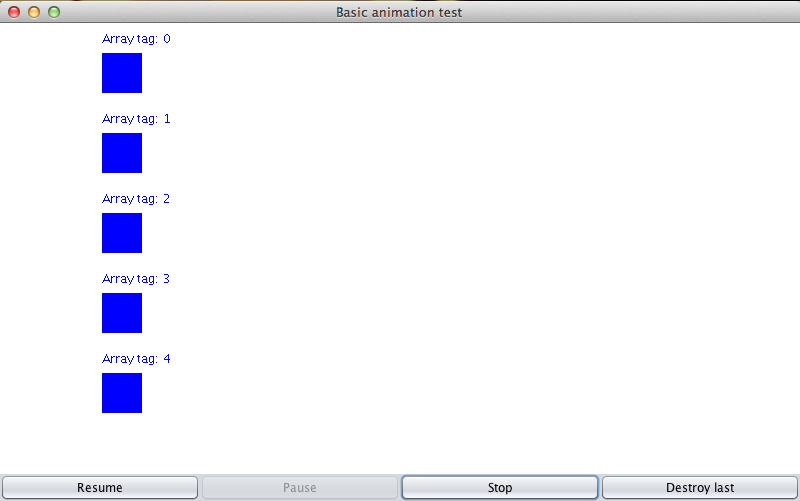
\includegraphics[width=\textwidth]{images/firstPrototype.png}
\end{center}
\caption{The first demonstration, produced by Andrew}
\label{fig:firstPrototype}
\end{figure}

While this was a good initial step, we did not have any obvious way to implement Steps, in a sense where multiple Animations could be assigned to one step and we could navigate through these steps back and forth. Therefore both Andrew and Arthur Bigeard started looking into it.

\begin{figure}
\begin{center}
\begin{verbatim}
public void timingEvent(Animator source, double fraction){
    boolean done = false;
    if(anArr.getToDo().size() > 0){
        Step[] steps = new Step[anArr.getToDo().peek().length];
        System.arraycopy(anArr.getToDo().peek(), 0, steps, 0, steps.length);

        for(int i = 0; i < steps.length; i++){                    
            Rectangle rect = rect_list[steps[i].getIndex()].getRec();
            double x = steps[i].getX();
            double y = steps[i].getY();
            double stepX = rect.getX();
            double stepY = rect.getY();
            if(y != stepY){
                if(Math.abs(x - stepX) < 50){
                    if(y > stepY){
                        rect_list[steps[i].getIndex()].getRec().x += 1;
                    }
                    else{
                        rect_list[steps[i].getIndex()].getRec().x -= 1;
                    }
                }
                else{
                    if(y > stepY){
                        rect_list[steps[i].getIndex()].getRec().y += 1;
                    }
                    else{
                        rect_list[steps[i].getIndex()].getRec().y -= 1;
                    }
                }
            }
            else{
                if(x > stepX){
                    rect_list[steps[i].getIndex()].getRec().x += 1;
                }
                else{
                    rect_list[steps[i].getIndex()].getRec().x -= 1;
                }
            }
            if(y == stepY && x == stepX){
                done = true;
                anArr.getToDo().poll();
                anArr.getDone().add(steps);
                break;
            }
        }
        repaint();              

    }
\end{verbatim}
\end{center}
\caption{Arthur example code making an animated change in coordinates}
\label{fig:arthurPrototype}
\end{figure}

Andrew had no real suggestions and Arthur’s prototype implementation seemed: 
\begin{itemize}
	\item too complex (a swap of 2 rectangles was over 50 lines long \ref{fig:arthurPrototype})
	\item impractical to use (it didn’t have any way to step back and forth through the animation) 
	\item it had a performance overhead (all Animator objects were running continuously, until the whole animation was stopped)
\end{itemize}
It had a few good points though: 
\begin{itemize}
	\item it was done on a low level (so the how-to part was obvious if you understood the code) 
	\item it was not storing too much information (thus it did not really have a memory overhead). 
\end{itemize}
But this was not what we wanted – the most important thing for us was the stepping back and forth functionality.  Therefore I started looking into it as well.

During my research of the Timing Framework I found out that we could add triggers, which would start an animation, to a button or to another animation, which would start another animation when it stops or starts running \cite{website:TimingFrameworkDemo}. Thus, triggers seemed like a great tool for linking multiple animations into one Step, linking steps and making a continuous animation.

\begin{figure}
\begin{center}
\begin{verbatim}
s.addAnimator(new Animator.Builder().setDuration(time, TimeUnit.MILLISECONDS)
	.build(), nextBtn);

s.getLastAnimator().addTarget(PropertySetter.getTarget(rect_list.get(b), 
	"currentX", rect_list.get(b).getRec().x, rect_list.get(a).getRec().x));}
\end{verbatim}
\end{center}
\caption{My example code making an animated change in coordinates}
\label{fig:gPrototype}
\end{figure}

I still wanted to find a way to make a change of a rectangle (or any other object) property easy to manage. Looking through the Demos I also found that I could use Targets and PropertySetters to do this in just a few lines of code \ref{fig:gPrototype}, which seemed great. But it only allowed us to change a property, which was numerical (like coordinates or colors) – it didn’t allow us to change all the properties of the object, like the labels of rectangles. To solve this issue, I researched further and found that we can create a class, which would implement a TimingTarget interface and its begin(), end(), repeat() and reverse() methods. Therefore, to solve the issue of changing the labels of rectangles I created a new class called ChangeLabel, which implemented a TimingTarget interface, its begin(), end(), repeat() and reverse() methods, and added a change of String variable just inside its begin method. This approach seemed great, because:
\begin{itemize}
	\item we can change any property of an object or do pretty much anything when that TimingTarget is called
	\item it is attached to each Animator object, so we do not have to worry about storing the TimingTargets anywhere
	\item it is efficient performance wise, because these TimingTargets are only executed, when the Animator object is
	\item it is easy to use, implement and understand
\end{itemize}

Therefore, the end result of my prototype was:
\begin{itemize}
	\item a list of steps
	\item an array of rectangles and their coordinates at each step
	\item an ability to either step back and forth through the animation by using buttons or see a continuous animation (and it was either that or that)
\end{itemize}

After looking through both my and Arthurs prototypes, we decided to merge the good parts of each: we kept most of my prototype, but reduced the amount of data stored for each Step, in particular, we made it so it would only store the details of the changed object before the change, rather than the details of all the objects.

The only issue left then, was the ability to have both step-by-step and continuous animations and allow the user to switch between them at any point of time, but this was not a big issue, since I just used a similar approach I used with ChangeLabel class:
\begin{enumerate}
	\item I created a new class, called ContinuousAnimation, which was also implementing the TimingTarget interface
	\item introduced a boolean variable called continuousAnimation, which was keeping record of whether the animation was in step-by-step or continuous mode
	\item made it so that the begin method in ContinuousAnimation would execute different actions according to the boolean continuousAnimation variable value:
	\begin{itemize}
		\item If true, Trigger the next Step
		\item If false, do nothing
	\end{itemize}
\end{enumerate}

\subsubsection{Refactoring}

Our first common implementation that we were using for development was coupled too much with AnimatedArray data structure and was not flexible at all. This became obvious, when we started implementing our AnimatedLinkedList. When we wanted to make our API to animate an AnimatedLinkedList instead of AnimatedArray, we had to change multiple classes, including Rect, ContinuousAnimation and ChangeLabel \ref{fig:coupling}. This was due to no polymorphism in our design.

\begin{figure}
\begin{center}
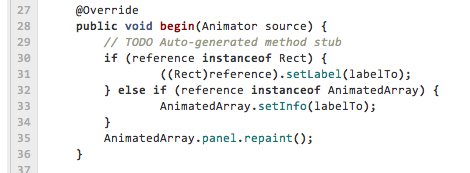
\includegraphics[width=\textwidth]{images/coupling.png}
\end{center}
\caption{ChangeLabel begin method dependency on AnimatedArray}
\label{fig:coupling}
\end{figure}

After doing our Professional Software Development 3 (PSD3) D7 deliverable (which was implementation of an Internship Management System we were designing the entire first semester), I have learned how to structure software better and how we can split code into components in Java. Therefore it was time for refactoring.

One of the first things I did was to create a separate package for each data structure. This lead to 4 additional packages being created:
\begin{itemize} 
	\item AnimatedArray
	\item AnimatedBinaryTree
	\item AnimatedDataStructure
	\item AnimatedLinkedList
\end{itemize}
Each package is supposed to keep classes relevant only to its data structure, apart from AnimatedDataStructure package, which keeps classes that are relevant to all data structures.

I also completely separated the GUI from the rest of the code and created a class called setupGUI.

\begin{figure}
\begin{center}
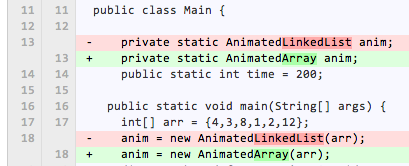
\includegraphics[width=\textwidth]{images/changeStructure.png}
\end{center}
\caption{Changing animation to animate a different data structure}
\label{fig:changeStructure}
\end{figure}

The next thing I did was to create a public interface AnimatedDataStructure, which is how we solved the issue I mentioned in the first paragraph. Rect, ContinuousAnimation, ChangeLabel and setupGUI are all expecting an AnimatedDataStructure variable now and all data structures are just implementing this interface. Therefore it does not matter which data structure we use, the common classes (which are in AnimatedDataStructure package) work for all of them. The interface itself also brought common method names and some structure. Another good thing is that now, we only need to change 2 things in the Main class if we want to work with a different data structure: the data structure class name and then the constructor method call \ref{fig:changeStructure}. This did bring in some repetitive methods, like getNextButton(), which are being repeated in all data structures, but could be solved by introducing another abstract class, which would be implementing the AnimatedDataStructure interface and have all of these repetitive methods and then making all data structure classes extend this new abstract class.

All of the above solutions introduced basic polymorphism to our software and solved quite a lot of development issues as well as made it easier to develop and manage the code for future developers (if there are going to be any). While doing all of the above, parts of unneccessary code were removed or changed as well.

\subsection{Liam Bell}

%==============================================================================
\chapter{Evaluation}

We evaluated the project by...

%==============================================================================
\chapter{Conclusion}

ASD

%==============================================================================
\section{Contributions}
\subsection{Arthur Bigeard}
\subsection{Alexander Ferguson}
\subsection{Andrew Gibson}
\subsection{Gediminas Leikus}
\subsection{Liam Bell}

%==============================================================================
\bibliographystyle{plain}
\bibliography{example}
\end{document}
